% Options for packages loaded elsewhere
\PassOptionsToPackage{unicode}{hyperref}
\PassOptionsToPackage{hyphens}{url}
%
\documentclass[
  12pt,
]{article}
\usepackage{lmodern}
\usepackage{amssymb,amsmath}
\usepackage{ifxetex,ifluatex}
\ifnum 0\ifxetex 1\fi\ifluatex 1\fi=0 % if pdftex
  \usepackage[T1]{fontenc}
  \usepackage[utf8]{inputenc}
  \usepackage{textcomp} % provide euro and other symbols
\else % if luatex or xetex
  \usepackage{unicode-math}
  \defaultfontfeatures{Scale=MatchLowercase}
  \defaultfontfeatures[\rmfamily]{Ligatures=TeX,Scale=1}
\fi
% Use upquote if available, for straight quotes in verbatim environments
\IfFileExists{upquote.sty}{\usepackage{upquote}}{}
\IfFileExists{microtype.sty}{% use microtype if available
  \usepackage[]{microtype}
  \UseMicrotypeSet[protrusion]{basicmath} % disable protrusion for tt fonts
}{}
\makeatletter
\@ifundefined{KOMAClassName}{% if non-KOMA class
  \IfFileExists{parskip.sty}{%
    \usepackage{parskip}
  }{% else
    \setlength{\parindent}{0pt}
    \setlength{\parskip}{6pt plus 2pt minus 1pt}}
}{% if KOMA class
  \KOMAoptions{parskip=half}}
\makeatother
\usepackage{xcolor}
\IfFileExists{xurl.sty}{\usepackage{xurl}}{} % add URL line breaks if available
\IfFileExists{bookmark.sty}{\usepackage{bookmark}}{\usepackage{hyperref}}
\hypersetup{
  pdftitle={Exercise 2 Solutions},
  pdfauthor={Ian McCarthy, Econ 771},
  hidelinks,
  pdfcreator={LaTeX via pandoc}}
\urlstyle{same} % disable monospaced font for URLs
\usepackage[left=2cm,right=2cm,top=1cm,bottom=2cm]{geometry}
\usepackage{color}
\usepackage{fancyvrb}
\newcommand{\VerbBar}{|}
\newcommand{\VERB}{\Verb[commandchars=\\\{\}]}
\DefineVerbatimEnvironment{Highlighting}{Verbatim}{commandchars=\\\{\}}
% Add ',fontsize=\small' for more characters per line
\usepackage{framed}
\definecolor{shadecolor}{RGB}{248,248,248}
\newenvironment{Shaded}{\begin{snugshade}}{\end{snugshade}}
\newcommand{\AlertTok}[1]{\textcolor[rgb]{0.94,0.16,0.16}{#1}}
\newcommand{\AnnotationTok}[1]{\textcolor[rgb]{0.56,0.35,0.01}{\textbf{\textit{#1}}}}
\newcommand{\AttributeTok}[1]{\textcolor[rgb]{0.77,0.63,0.00}{#1}}
\newcommand{\BaseNTok}[1]{\textcolor[rgb]{0.00,0.00,0.81}{#1}}
\newcommand{\BuiltInTok}[1]{#1}
\newcommand{\CharTok}[1]{\textcolor[rgb]{0.31,0.60,0.02}{#1}}
\newcommand{\CommentTok}[1]{\textcolor[rgb]{0.56,0.35,0.01}{\textit{#1}}}
\newcommand{\CommentVarTok}[1]{\textcolor[rgb]{0.56,0.35,0.01}{\textbf{\textit{#1}}}}
\newcommand{\ConstantTok}[1]{\textcolor[rgb]{0.00,0.00,0.00}{#1}}
\newcommand{\ControlFlowTok}[1]{\textcolor[rgb]{0.13,0.29,0.53}{\textbf{#1}}}
\newcommand{\DataTypeTok}[1]{\textcolor[rgb]{0.13,0.29,0.53}{#1}}
\newcommand{\DecValTok}[1]{\textcolor[rgb]{0.00,0.00,0.81}{#1}}
\newcommand{\DocumentationTok}[1]{\textcolor[rgb]{0.56,0.35,0.01}{\textbf{\textit{#1}}}}
\newcommand{\ErrorTok}[1]{\textcolor[rgb]{0.64,0.00,0.00}{\textbf{#1}}}
\newcommand{\ExtensionTok}[1]{#1}
\newcommand{\FloatTok}[1]{\textcolor[rgb]{0.00,0.00,0.81}{#1}}
\newcommand{\FunctionTok}[1]{\textcolor[rgb]{0.00,0.00,0.00}{#1}}
\newcommand{\ImportTok}[1]{#1}
\newcommand{\InformationTok}[1]{\textcolor[rgb]{0.56,0.35,0.01}{\textbf{\textit{#1}}}}
\newcommand{\KeywordTok}[1]{\textcolor[rgb]{0.13,0.29,0.53}{\textbf{#1}}}
\newcommand{\NormalTok}[1]{#1}
\newcommand{\OperatorTok}[1]{\textcolor[rgb]{0.81,0.36,0.00}{\textbf{#1}}}
\newcommand{\OtherTok}[1]{\textcolor[rgb]{0.56,0.35,0.01}{#1}}
\newcommand{\PreprocessorTok}[1]{\textcolor[rgb]{0.56,0.35,0.01}{\textit{#1}}}
\newcommand{\RegionMarkerTok}[1]{#1}
\newcommand{\SpecialCharTok}[1]{\textcolor[rgb]{0.00,0.00,0.00}{#1}}
\newcommand{\SpecialStringTok}[1]{\textcolor[rgb]{0.31,0.60,0.02}{#1}}
\newcommand{\StringTok}[1]{\textcolor[rgb]{0.31,0.60,0.02}{#1}}
\newcommand{\VariableTok}[1]{\textcolor[rgb]{0.00,0.00,0.00}{#1}}
\newcommand{\VerbatimStringTok}[1]{\textcolor[rgb]{0.31,0.60,0.02}{#1}}
\newcommand{\WarningTok}[1]{\textcolor[rgb]{0.56,0.35,0.01}{\textbf{\textit{#1}}}}
\usepackage{longtable,booktabs}
% Correct order of tables after \paragraph or \subparagraph
\usepackage{etoolbox}
\makeatletter
\patchcmd\longtable{\par}{\if@noskipsec\mbox{}\fi\par}{}{}
\makeatother
% Allow footnotes in longtable head/foot
\IfFileExists{footnotehyper.sty}{\usepackage{footnotehyper}}{\usepackage{footnote}}
\makesavenoteenv{longtable}
\usepackage{graphicx}
\makeatletter
\def\maxwidth{\ifdim\Gin@nat@width>\linewidth\linewidth\else\Gin@nat@width\fi}
\def\maxheight{\ifdim\Gin@nat@height>\textheight\textheight\else\Gin@nat@height\fi}
\makeatother
% Scale images if necessary, so that they will not overflow the page
% margins by default, and it is still possible to overwrite the defaults
% using explicit options in \includegraphics[width, height, ...]{}
\setkeys{Gin}{width=\maxwidth,height=\maxheight,keepaspectratio}
% Set default figure placement to htbp
\makeatletter
\def\fps@figure{htbp}
\makeatother
\setlength{\emergencystretch}{3em} % prevent overfull lines
\providecommand{\tightlist}{%
  \setlength{\itemsep}{0pt}\setlength{\parskip}{0pt}}
\setcounter{secnumdepth}{-\maxdimen} % remove section numbering
\usepackage{setspace}
\usepackage{titlesec}
\titlespacing{\title}{0pt}{\parskip}{-\parskip}
\titlespacing{\section}{0pt}{12pt plus 2pt minus 1pt}{0pt plus 1pt minus 1pt}
\titlespacing{\subsection}{0pt}{12pt plus 2pt minus 1pt}{0pt plus 1pt minus 1pt}
\titlespacing{\subsubsection}{0pt}{12pt plus 2pt minus 1pt}{0pt plus 1pt minus 1pt}
\usepackage{float}
\usepackage{booktabs}
\usepackage{longtable}
\usepackage{array}
\usepackage{multirow}
\usepackage{wrapfig}
\usepackage{float}
\usepackage{colortbl}
\usepackage{pdflscape}
\usepackage{tabu}
\usepackage{threeparttable}
\usepackage{threeparttablex}
\usepackage[normalem]{ulem}
\usepackage{makecell}
\usepackage{xcolor}
\newlength{\cslhangindent}
\setlength{\cslhangindent}{1.5em}
\newenvironment{cslreferences}%
  {\setlength{\parindent}{0pt}%
  \everypar{\setlength{\hangindent}{\cslhangindent}}\ignorespaces}%
  {\par}

\title{Exercise 2 Solutions}
\author{Ian McCarthy, Econ 771}
\date{Fall 2020}

\begin{document}
\maketitle

\setstretch{1.5}

\hypertarget{overview}{%
\section{Overview}\label{overview}}

This document lays out my approach to addressing the questions in Exercise 2. There are lots of ways to answer these problems and build the data, especially in \texttt{R}! My way of answering the questions is just one of many.

I also have a particular workflow that you may or may not choose to adopt. That workflow is to do all of my analysis seperately from my markdown document. I really don't like seeing huge markdown documents constantly going in and out of data work and discussion. It's also not feasible to work with really large data within the markdown document. So, I do all of the analysis, remove any large objects (including the data), keep only the relevant objects for the final markdown (figures, tables, specific numbers or statistics), and then save the workspace. Then I load the workspace into my markdown document.

\hypertarget{data}{%
\section{Data}\label{data}}

Before we get into the specific questions for this assignment, let's briefly go through the data. My code files for the benchmark data, penetration data, and AHRF data are included in the classroom repo under the filenames \emph{1\_benchmark.R}, \emph{2\_penetration.R}, and \emph{3\_ahrf.R}.

\hypertarget{benchmark-data}{%
\subsubsection{Benchmark data}\label{benchmark-data}}

MA benchmarks reflect a payment that CMS sets for each enrollee of a MA plan. The payment varied by county. CMS doesn't actually pay this rate to each plan - the final payment depends on the plan's ``bid''. This is not a ``bid'' in the standard auction sense. It's just the terminology used by CMS. Essentially, each plan sets their premium, and if the premium is below the benchmark rate, CMS pays the plan a risk-adjusted benchmark rate for each enrollee, and plans must use the bid-benchmark differential to expand plan benefits. If the premium exceeds the benchmark rate, then CMS pays the plan the benchmark rate, and the plan passes the bid-benchmark differential onto the enrollee in the form of a montnly premium.

Beginning in 2012, benchmark payments also vary by the star rating of each MA plan. I didn't worry about this for our assignment. Instead, I just set the county-level benchmark rate equal to the benchmark rate for a 3-star plan, as follows:

\setstretch{1}

\begin{Shaded}
\begin{Highlighting}[]
  \KeywordTok{mutate}\NormalTok{(}\DataTypeTok{bench\_pay=}
    \KeywordTok{case\_when}\NormalTok{(}
\NormalTok{      year}\OperatorTok{\textless{}}\DecValTok{2012} \OperatorTok{\textasciitilde{}}\StringTok{ }\NormalTok{risk\_ab,}
\NormalTok{      year}\OperatorTok{\textgreater{}=}\DecValTok{2012} \OperatorTok{\&}\StringTok{ }\NormalTok{year}\OperatorTok{\textless{}}\DecValTok{2015} \OperatorTok{\textasciitilde{}}\StringTok{ }\NormalTok{risk\_star3,}
\NormalTok{      year}\OperatorTok{\textgreater{}=}\DecValTok{2015} \OperatorTok{\textasciitilde{}}\StringTok{ }\NormalTok{risk\_bonus0,}
      \OtherTok{TRUE} \OperatorTok{\textasciitilde{}}\StringTok{ }\OtherTok{NA\_real\_}
\NormalTok{    ))}
\end{Highlighting}
\end{Shaded}

\setstretch{1.5}

\hypertarget{penetration-data}{%
\subsubsection{Penetration data}\label{penetration-data}}

Enrollments for MA plans are published at the plan/county/year/month level. But in reality, plan enrollments don't change much across months in the same year. For the most part, enrollees are locked into whatever plan thay choose for the year. There are exceptions, and anyone can drop a plan if they choose, but there are restrictions to which plans people can switch into outside of the open enrollment period. To make things easier, I just took the penetration data for December of each year for this exercise. In my full \href{https://github.com/imccart/Medicare-Advantage}{MA repo}, there is some code to work with each month and average enrollments over the year if you are so inclined.

\hypertarget{ahrf-data}{%
\subsubsection{AHRF data}\label{ahrf-data}}

The AHRF data are easy to download but can be tricky to read into R. The best solution is to use the \texttt{SAScii} package, which allows you to read in the full ascii (.asc) file using the .sas input file provided as part of the data documentation. It is a slow process but works just fine. Then you just need to identify the variable of interest using the technical documents (\emph{F15299} in our case).

\hypertarget{final-dataset}{%
\subsubsection{Final dataset}\label{final-dataset}}

Once you have the benchmark, penetration, and AHRF data together, you just have to merge them all. The easiest way to do this in our case is to merge on SSA and Year. Here's my code to merge the three datasets:

\setstretch{1}

\begin{Shaded}
\begin{Highlighting}[]
\NormalTok{full.data \textless{}{-}}\StringTok{ }\NormalTok{ma.penetration.data }\OperatorTok{\%\textgreater{}\%}\StringTok{ }
\StringTok{  }\KeywordTok{left\_join}\NormalTok{(ma.benchmark.data }\OperatorTok{\%\textgreater{}\%}\StringTok{ }\KeywordTok{select}\NormalTok{(year, ssa, bench\_pay, }\KeywordTok{starts\_with}\NormalTok{(}\StringTok{"risk"}\NormalTok{)),}
            \DataTypeTok{by=}\KeywordTok{c}\NormalTok{(}\StringTok{"ssa"}\NormalTok{,}\StringTok{"year"}\NormalTok{)) }\OperatorTok{\%\textgreater{}\%}
\StringTok{  }\KeywordTok{left\_join}\NormalTok{(ahrf.data }\OperatorTok{\%\textgreater{}\%}\StringTok{ }\KeywordTok{select}\NormalTok{(year, ssa, medicare\_ffs\_exp), }
            \DataTypeTok{by=}\KeywordTok{c}\NormalTok{(}\StringTok{"ssa"}\NormalTok{,}\StringTok{"year"}\NormalTok{)) }\OperatorTok{\%\textgreater{}\%}
\StringTok{  }\KeywordTok{filter}\NormalTok{(year}\OperatorTok{\textgreater{}=}\DecValTok{2010}\NormalTok{,}
  \KeywordTok{complete.cases}\NormalTok{(bench\_pay, medicare\_ffs\_exp, penetration))}
\end{Highlighting}
\end{Shaded}

\setstretch{1.5}

Note that I limit the data to ``complete cases'' (i.e., units of observation in which all of the main variables are observed in the data). This is a good rule-of-thumb for any empirical work because it ensures that you're working with the same sample across different analyses; although it's not always possible if you're working with lots of outcomes.

\hypertarget{question-and-answers}{%
\section{Question and Answers}\label{question-and-answers}}

\hypertarget{question-1.}{%
\subsubsection{Question 1.}\label{question-1.}}

\textbf{Provide and discuss a table of simple summary statistics showing the mean, standard deviation, min, and max of the Medicare Advantage penetration rate, benchmark payments, and utilization measures.}

Table \ref{tab:sum-stats} presents the mean, standard deviation, min, and max of the relevant variables. Note the

\hypertarget{question-2.}{%
\subsubsection{Question 2.}\label{question-2.}}

\textbf{Plot the mean county-level utilization against the mean MA penetration rate over time.}

Figure \ref{fig:scatter} presents the MA penetration and Medicare expenditures, averaged across counties by year.

\hypertarget{question-3}{%
\subsubsection{Question 3}\label{question-3}}

\textbf{Using the MA benchmark as an IV for MA penetration rates, estimate the effects of MA penetration on utilization. This is analogous to the specification in Baicker, Chernew, and Robbins (2013).}

I'll focus on a very simple specification here, using only the instrument (MA benchmark rates), the endogenous variable (MA penetration rate), and some county/year fixed effects. The syntax for this in \texttt{R} is:

\begin{Shaded}
\begin{Highlighting}[]
\KeywordTok{felm}\NormalTok{(medicare\_ffs\_exp }\OperatorTok{\textasciitilde{}}\StringTok{ }\DecValTok{0} \OperatorTok{|}\StringTok{ }\NormalTok{year }\OperatorTok{+}\StringTok{ }\NormalTok{ssa }\OperatorTok{|}\StringTok{ }\NormalTok{(penetration }\OperatorTok{\textasciitilde{}}\StringTok{ }\NormalTok{bench\_pay) }\OperatorTok{|}\StringTok{ }\NormalTok{ssa, }
     \DataTypeTok{data=}\NormalTok{full.data)}
\end{Highlighting}
\end{Shaded}

The IV results are presented in Table \ref{tab:iv1}.

\hypertarget{question-4}{%
\subsubsection{Question 4}\label{question-4}}

\textbf{Present the ``first stage'' and ``reduced form'' results of your IV estimates in Part 3.}

Quick refresher: The first stage is just the regression of the endogenous variable on all of the exogneous variables and your instrument, and the reduced form is a regression of your outcome on all the exogenous variables and the instrument. Recall that an IV estimate is just the ratio of the reduced form and the first stage, so it's good to look at these things specifically. The results are presented in Table \ref{tab:iv2}.

\hypertarget{question-5}{%
\subsubsection{Question 5}\label{question-5}}

\textbf{Present selected specification/robustness checks of your IV and discuss two weaknesses of this identification strategy.}

There's no wrong answer here. I just want you to think critically about our identification and data. I'm going to check two issues:

\emph{1. Are the results sensitive to the use of the 3-star benchmark rate?}

I replaced the benchmark payment rate with the 3.5-star benchmark payment rate just to see how the results change. Coefficient estimates are presented in Table \ref{tab:sens1}.

\emph{2. Are the results sensitive to outliers in Medicare FFS expenditures?}

Outliers are known to be a potentially major problem in any IV estimate. To examine the sensitivity of results to such outliers, I consider the ``robust IV'' estimator from Freue, Ortiz-Molina, and Zamar (2013). This is easily implemented with the \texttt{R} package that accompanies their paper, \texttt{riv}.

This ``robust instrumental variables'' estimator uses a ``robust multivariate location and scatter S-estimator'' and ultimately provides an IV estimate that is resilient to the presence of outliers (much more resilient than the standard IV). The ``S-estimator'' (I think) just denotes that we are ``simultaneously'' estimating both a location (measure of centrality) vector and scatter (measure of dispersion), but we are doing so with a slightly different objective function other than the sum of squared errors.

In this case, you have to do a little extra work to fully replicate our original results. That's because we have lots of fixed effects\ldots trying to include all of them explicitly as dummies in the RIV estimator will take forever. We can do this by taking advantage of the Frisch-Waugh-Lovell theorem and partialling out all of the fixed effects (year and ssa) from each variable of interest. In this case, we just estimate a linear regression of each variable on all of the fixed effects, take the residuals, and then run the RIV on the residualized values. Here's the code to do it:

\setstretch{1}

\begin{Shaded}
\begin{Highlighting}[]
\NormalTok{y.resid \textless{}{-}}\StringTok{ }\KeywordTok{lm}\NormalTok{(medicare\_ffs\_exp }\OperatorTok{\textasciitilde{}}\StringTok{ }\KeywordTok{factor}\NormalTok{(year) }\OperatorTok{+}\StringTok{ }\KeywordTok{factor}\NormalTok{(ssa),}
                \DataTypeTok{data=}\NormalTok{riv.data)}
\NormalTok{x.resid \textless{}{-}}\StringTok{ }\KeywordTok{lm}\NormalTok{(penetration }\OperatorTok{\textasciitilde{}}\StringTok{ }\KeywordTok{factor}\NormalTok{(year) }\OperatorTok{+}\StringTok{ }\KeywordTok{factor}\NormalTok{(ssa),}
                \DataTypeTok{data=}\NormalTok{riv.data)}
\NormalTok{z.resid \textless{}{-}}\StringTok{ }\KeywordTok{lm}\NormalTok{(bench\_pay }\OperatorTok{\textasciitilde{}}\StringTok{ }\KeywordTok{factor}\NormalTok{(year) }\OperatorTok{+}\StringTok{ }\KeywordTok{factor}\NormalTok{(ssa),}
                \DataTypeTok{data=}\NormalTok{riv.data)}

\NormalTok{riv.data \textless{}{-}}\StringTok{ }\NormalTok{riv.data }\OperatorTok{\%\textgreater{}\%}
\StringTok{  }\KeywordTok{spread\_residuals}\NormalTok{(y.resid, x.resid, z.resid) }\OperatorTok{\%\textgreater{}\%}
\StringTok{  }\KeywordTok{filter}\NormalTok{(}\KeywordTok{complete.cases}\NormalTok{(y.resid, x.resid, z.resid))}


\NormalTok{Y \textless{}{-}}\StringTok{ }\KeywordTok{as.matrix}\NormalTok{(full.data[,}\DecValTok{30}\NormalTok{])}
\NormalTok{Xend \textless{}{-}}\StringTok{ }\KeywordTok{as.matrix}\NormalTok{(full.data[,}\DecValTok{31}\NormalTok{])}
\NormalTok{Zinst \textless{}{-}}\StringTok{ }\KeywordTok{as.matrix}\NormalTok{(full.data[,}\DecValTok{32}\NormalTok{])}

\NormalTok{robust.iv1 \textless{}{-}}\StringTok{ }\KeywordTok{riv}\NormalTok{(Y, Xend, }\DataTypeTok{Xex=}\OtherTok{NULL}\NormalTok{, Zinst, }\DataTypeTok{method=}\StringTok{"classical"}\NormalTok{)}
\NormalTok{robust.iv2 \textless{}{-}}\StringTok{ }\KeywordTok{riv}\NormalTok{(Y, Xend, }\DataTypeTok{Xex=}\OtherTok{NULL}\NormalTok{, Zinst)}
\end{Highlighting}
\end{Shaded}

\setstretch{1.5}

Note that the RIV package is a little clunky. To accommodate the package, we need to drop incomplete cases (rows with any missing values). I've also explicitly defined the variables/covariates as their own matrices.

The coefficient estimate for MA penetration on Medicare payments using the default \emph{S}-estimator is -86.48. Note that this is quite a bit larger than our original estimate of -46.164. Just to check, I also compared the ``partialled-out'' version of our estimator with a classical IV. This is the \texttt{robust.iv1} object in the above code. This should yield the same point estimate as the standard IV estimate earlier. Thankfully, they are the same.

\newpage
\setstretch{1}

\hypertarget{tables-and-figures}{%
\section{Tables and Figures}\label{tables-and-figures}}

\begin{table}[h]

\caption{\label{tab:sum-stats}Summary Statistics}
\centering
\begin{tabular}[t]{lrrrr}
\toprule
Variable & Mean & Std. Dev. & Min & Max\\
\midrule
MA Share & 19.09 & 12.88 & 0.17 & 213.60\\
Benchmark Pymt & 795.22 & 71.63 & 280.09 & 1,358.13\\
FFS Expenditure & 9,747.87 & 1,169.40 & 4,876.11 & 20,451.58\\
\bottomrule
\end{tabular}
\end{table}

\newpage

\begin{table}[H] \centering 
  \caption{IV Results} 
  \label{tab:iv1} 
\begin{tabular}{@{\extracolsep{5pt}}lc} 
\\[-1.8ex]\hline 
\hline \\[-1.8ex] 
 & \multicolumn{1}{c}{\textit{Dependent variable:}} \\ 
\cline{2-2} 
\\[-1.8ex] & Medicare Exp \\ 
\hline \\[-1.8ex] 
 MA Share & $-$46.164$^{*}$ \\ 
  & (25.238) \\ 
  & \\ 
\hline \\[-1.8ex] 
Observations & 18,352 \\ 
R$^{2}$ & 0.785 \\ 
Adjusted R$^{2}$ & 0.742 \\ 
Residual Std. Error & 593.073 (df = 15245) \\ 
\hline 
\hline \\[-1.8ex] 
\textit{Note:}  & \multicolumn{1}{r}{$^{*}$p$<$0.1; $^{**}$p$<$0.05; $^{***}$p$<$0.01} \\ 
\end{tabular} 
\end{table}

\newpage

\begin{table}[H] \centering 
  \caption{First Stage and Reduced Form IV Results} 
  \label{tab:iv2} 
\begin{tabular}{@{\extracolsep{5pt}}lcc} 
\\[-1.8ex]\hline 
\hline \\[-1.8ex] 
 & \multicolumn{2}{c}{\textit{Dependent variable:}} \\ 
\cline{2-3} 
\\[-1.8ex] & MA Share & Medicare Exp \\ 
\\[-1.8ex] & (1) & (2)\\ 
\hline \\[-1.8ex] 
 Benchmark Pymt & $-$0.011$^{***}$ & 0.510$^{**}$ \\ 
  & (0.002) & (0.258) \\ 
  & & \\ 
\hline \\[-1.8ex] 
Observations & 18,352 & 18,352 \\ 
R$^{2}$ & 0.947 & 0.797 \\ 
Adjusted R$^{2}$ & 0.937 & 0.755 \\ 
Residual Std. Error (df = 15245) & 3.238 & 577.475 \\ 
\hline 
\hline \\[-1.8ex] 
\textit{Note:}  & \multicolumn{2}{r}{$^{*}$p$<$0.1; $^{**}$p$<$0.05; $^{***}$p$<$0.01} \\ 
\end{tabular} 
\end{table}

\newpage

\begin{table}[H] \centering 
  \caption{Alternative IV Results} 
  \label{tab:sens1} 
\begin{tabular}{@{\extracolsep{5pt}}lccc} 
\\[-1.8ex]\hline 
\hline \\[-1.8ex] 
 & \multicolumn{3}{c}{\textit{Dependent variable:}} \\ 
\cline{2-4} 
\\[-1.8ex] & Medicare Exp & MA Share & Medicare Exp \\ 
\\[-1.8ex] & (1) & (2) & (3)\\ 
\hline \\[-1.8ex] 
 MA Share & $-$46.164$^{*}$ &  &  \\ 
  & (25.238) &  &  \\ 
  & & & \\ 
 Benchmark Pymt &  & $-$0.011$^{***}$ & 0.510$^{**}$ \\ 
  &  & (0.002) & (0.258) \\ 
  & & & \\ 
\hline \\[-1.8ex] 
Observations & 18,352 & 18,352 & 18,352 \\ 
R$^{2}$ & 0.785 & 0.947 & 0.797 \\ 
Adjusted R$^{2}$ & 0.742 & 0.937 & 0.755 \\ 
Residual Std. Error (df = 15245) & 593.073 & 3.238 & 577.475 \\ 
\hline 
\hline \\[-1.8ex] 
\textit{Note:}  & \multicolumn{3}{r}{$^{*}$p$<$0.1; $^{**}$p$<$0.05; $^{***}$p$<$0.01} \\ 
\end{tabular} 
\end{table}

\newpage

\begin{figure}
\centering
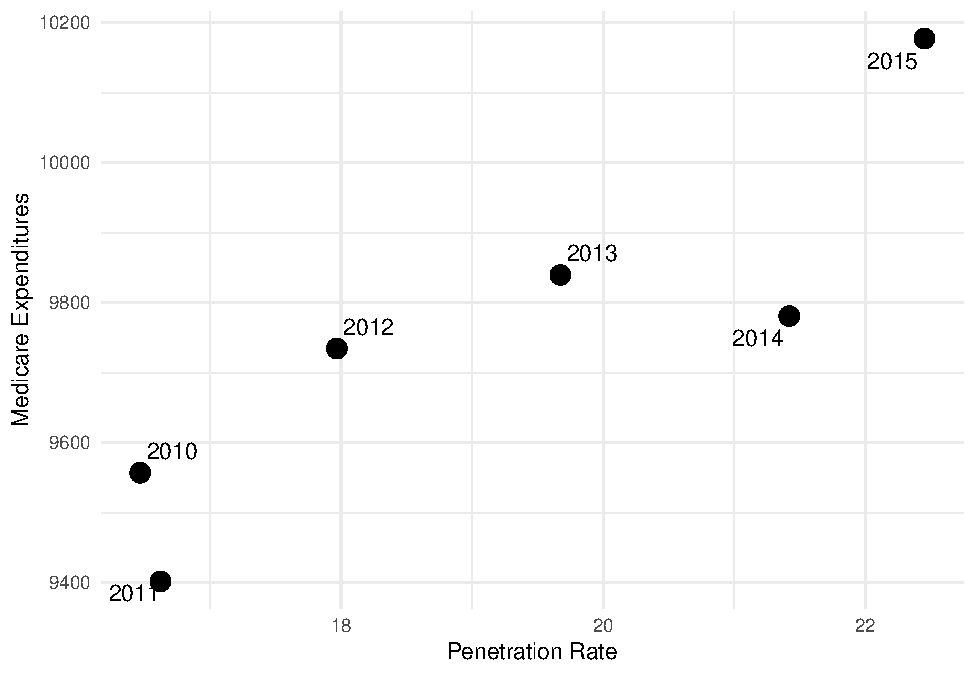
\includegraphics{solutions_files/figure-latex/scatter-1.pdf}
\caption{\label{fig:scatter}Mean MA penetration rates and payments by year}
\end{figure}

\newpage

\hypertarget{references}{%
\section*{References}\label{references}}
\addcontentsline{toc}{section}{References}

\hypertarget{refs}{}
\begin{cslreferences}
\leavevmode\hypertarget{ref-freue2013}{}%
Freue, Gabriela V Cohen, Hernan Ortiz-Molina, and Ruben H Zamar. 2013. ``A Natural Robustification of the Ordinary Instrumental Variables Estimator.'' \emph{Biometrics} 69 (3): 641--50.
\end{cslreferences}

\end{document}
